\chapter{Thème: Eponge de Menger}
{ }\hfill\textbf{Niveau:} Avancé\\ \\
Dans ce chapitre, nous allons construire un solide fractal appelé l'éponge de Menger. Voici les premières itérations pour contruire ce solide:
\begin{center}
\begin{minipage}{6cm}
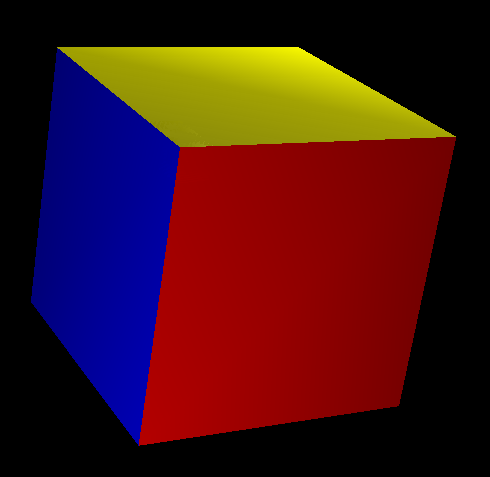
\includegraphics[width=6cm]{images/menger0.png}
\begin{center}
 \textbf{Etape 0}
\end{center}
\end{minipage}
\begin{minipage}{6cm}
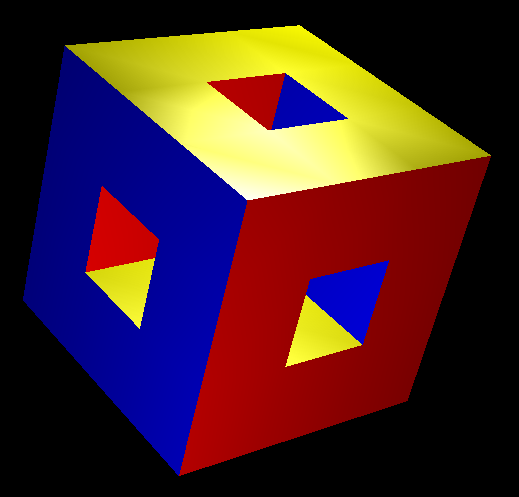
\includegraphics[width=6cm]{images/menger1.png}
\begin{center}
 \textbf{Etape 1}
\end{center}
\end{minipage}
\\
\begin{minipage}{6cm}
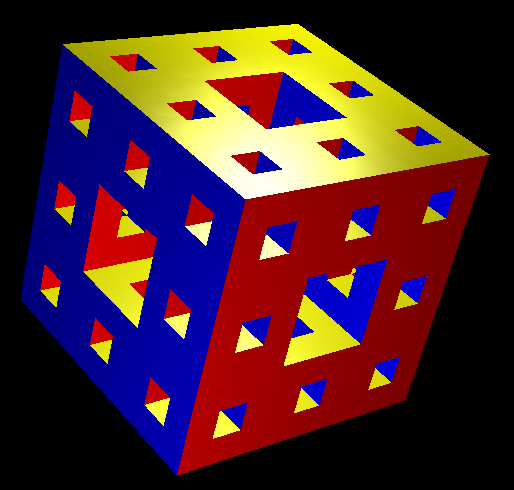
\includegraphics[width=6cm]{images/menger2.png}
\begin{center}
 \textbf{Etape 2}
\end{center}
\end{minipage}
\begin{minipage}{6cm}
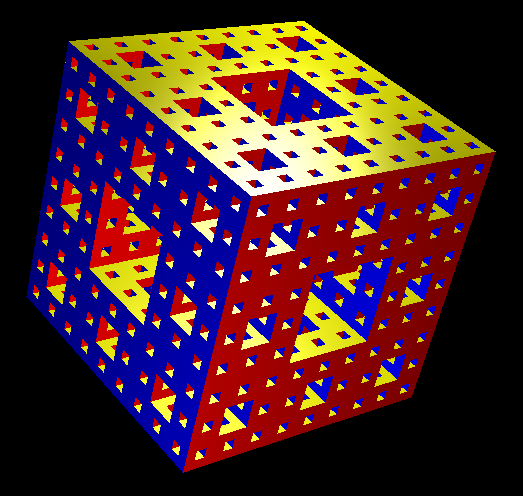
\includegraphics[width=6cm]{images/menger3.png}
\begin{center}
 \textbf{Etape 3}
\end{center}
\end{minipage}
\end{center}
Le chapitre se décompose en deux parties:
\begin{itemize}
 \item Tout d'abord, nous montrerons comment créer ce solide aisément en utilisant la récursivité.
 \item Dans un deuxième temps, on essaiera d'optimiser le tracé afin de tracer une éponge de Menger d'ordre~4.
\end{itemize}
\section{En utilisant la récursivité}
\noindent Considérons une éponge de menger d'ordre $n$ dont le côté mesure $L$.\\
\begin{center}
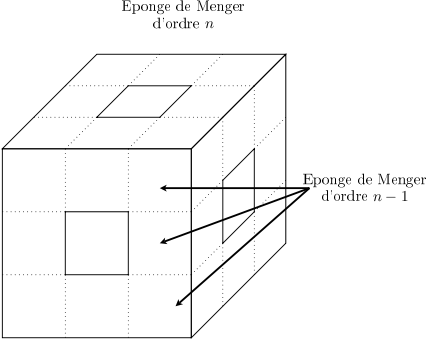
\includegraphics{images/menger-schema01.png}
\end{center}
Le schéma montre bien que cette éponge est constitué en fait de 20 éponges de Menger d'ordre $n-1$ ayant chacune un côté de $\dfrac{L}{3}$. La structure récursive de l'éponge est ainsi mise en évidence.\\ \\
\textbf{Le programme:}
\begin{verbatim}
# Commande principale: eponge 3
pour cube :l
si :compteur=10000 [vue3d]
# Couleur des faces latérales
soit "couleurs [jaune magenta cyan bleu]
# faces latérales
repete 4 [fcc exec item compteur :couleurs carre :l td 90 av  :l tg 90 rd 90]
# Dessous
fcc rouge pique 90 carre :l cabre 90
av :l pique 90 fcc vert carre :l cabre 90 re :l
fin

pour carre :c
donne "compteur :compteur+1
polydef
repete 4 [av :c td 90]
polyfin
fin

# Eponde de Menger 
# p: profondeur de récursivité
# l: Longueur du grand cube.
pour menger :l :p
si :p=0 [cube :l] [
  soit "p :p-1  
  soit "l :l/3
  #face avant
  repete 3 [menger :l :p av :l] re 3*:l
  td 90 av :l tg 90
  menger :l :p av 2*:l menger :l :p re 2*:l
  td 90 av :l tg 90
  repete 3 [menger :l :p av :l] re 3*:l
  #Côté droit 
 pique 90 av :l cabre 90 
  menger :l :p  av 2*:l menger :l :p re 2*:l
  pique 90 av :l cabre 90 
  repete 3 [menger :l :p av :l] re 3*:l
  tg 90 av :l td 90
  menger :l :p  av 2*:l menger :l :p re 2*:l
  tg 90 av :l td 90
  repete 3 [menger :l :p av :l] re 3*:l
  pique 90 re :l cabre 90
  menger :l :p  av 2*:l menger :l :p re 2*:l
   pique 90 re :l cabre 90
]
fin

pour eponge :p
ve ct donne "compteur 0 perspective fcfg 0 menger 800 :p 
tape [Nombre de polygone: ] ec :compteur 
vue3d
fin
\end{verbatim}
Ce programme comprend quatre procédures:
\begin{itemize}
 \item \texttt{carre :c}\\
Cette procédure trace un carré de côté \texttt{:c}. De plus, ce polygone est enregistré par le modeleur 3D. La variable \texttt{compteur} est chargée de dénombrer le nombre de polygones dessinés.
 \item \texttt{cube :l}\\
Cette procédure trace un cube de côté \texttt{:l}. Elle utilise bien sûr la procédure \texttt{carre}
 \item \texttt{menger :l :p}\\
Cette procédure est la clé du programme, elle dessine un motif de Menger d'ordre $p$ et dont le côté mesure $l$. Ce motif est créé de manière récursive de manière tout à fait naturelle en exploitant le schéma précédent.
 \item \texttt{eponge :p}\\
Cette procédure trace une eponge de Menger d'ordre $p$ et de côté 800 puis l'affiche dans le modeleur 3D.
\end{itemize}
\vfill
\pagebreak
\section{Deuxième approche: objectif solide d'ordre 4}
Le programme précédent a pour principal avantage d'exploiter la structure naturellement récursive du solide fractal. On peut noter que cette même méthode peut être réemployer pour générer d'autres solides fractals, ou plus simplement, d'autres courbes fractales. En tout cas, La conséquence immédiate de l'approche récursive est un code court et simple à comprendre. Malheureusement, on s'aperçoit qu'une éponge d'ordre 3 nécessite déjà 48 000 polygônes. Il faut alors régler la mémoire allouée à XLogo à 256 Mo dans le panneau des préférences pour que le programme puisse s'exécuter entièrement. \\ \\
Si l'on souhaite tracer une éponge de Menger d'ordre 4, on va vite être bloqué par un dépassement mémoire. Nous allons voir dans cette partie un programme basé sur un algorithme complètement différent, il permettra de créer une éponge de Menger d'ordre 0,1,2,3 ou 4.
\subsection{Le tapis de Sierpinski}
\noindent L'éponge de Menger est en fait la généralisation en 3 dimensions d'une figure du plan appelée le tapis de Sierpinski. Voici les premières itérations de cette figure:\\ \\
\begin{minipage}{4.5cm}
\begin{center}
 
\includegraphics[width=4.5cm]{images/carpet0.png}\\
\textbf{Etape 0}
\end{center}
\end{minipage}
\begin{minipage}{4.5cm}
\begin{center}
 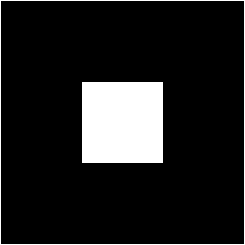
\includegraphics[width=4.5cm]{images/carpet1.png}\\
\textbf{Etape 1}
\end{center}
\end{minipage}
\begin{minipage}{4.5cm}
\begin{center}
 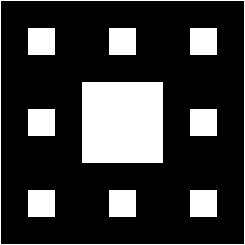
\includegraphics[width=4.5cm]{images/carpet2.png}\\
\textbf{Etape 2}
\end{center}
\end{minipage}
\begin{minipage}{4.5cm}
\begin{center}
 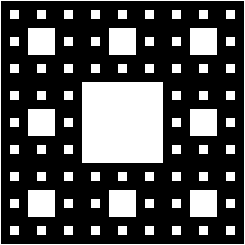
\includegraphics[width=4.5cm]{images/carpet3.png}\\
\textbf{Etape 3}
\end{center}
\end{minipage}\\ 
\vspace*{0.5cm}\\
Le motif présent sur chacune des faces d'une éponge de Menger d'ordre $p$ est un tapis de Sierpinski d'ordre $p$.
\subsection{Tracer un tapis de Sierpinski d'ordre $p$}
L'objectif est déjà de réussir à minimiser le nombre de polygônes nécessaires pour dessiner un tapis de Sierpinski. L'exemple suivant explique le procédé employé pour créer un tapis de Sierpinski d'ordre 3. Ici, le carré initial comporte donc $3^3=27$ lignes et 27 colonnes. On écrit en base 3 le numéro de chacune des lignes et de chacune des colonnes.
\begin{itemize}
 \item [\textbullet]\textbf{Première étape:} Pour toutes les lignes dont le numéro ne comporte aucun 1, on trace une ligne de 27 carreaux. Par symétrie, on effectue la même opération sur les colonnes.\\
\begin{center}
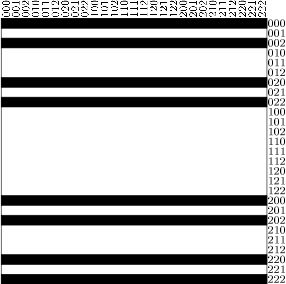
\includegraphics{images/menger-schema02.png}
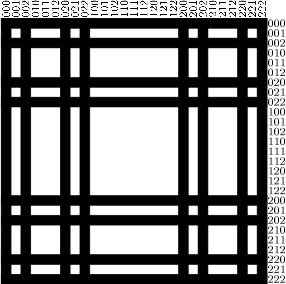
\includegraphics{images/menger-schema03.png}
\end{center}
\vspace{0.2cm}
\item [\textbullet] \textbf{Deuxième étape:} On s'intéresse à présent aux lignes dont le numéro comporte un seul 1 en première position. On trace successivement par alternance des rectangles de longueur 9 carreaux. On reporte alors cette opération sur les colonnes par symétrie .\\
\begin{center}
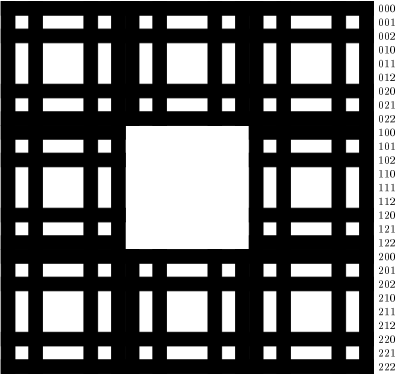
\includegraphics{images/menger-schema04.png}
\end{center} 
\item [\textbullet] \textbf{Troisième étape:} On s'intéresse à présent aux lignes dont le numéro comporte un seul 1 en deuxième position. On trace successivement par alternance des rectangles en suivant le schéma $[3\ 3\ 6\ 3\ 6\ 3\ 3]$. (3 carreaux tracés, 3 non tracés, 6 tracés etc...) On reporte alors par symétrie cette opération sur les colonnes.
\begin{center}
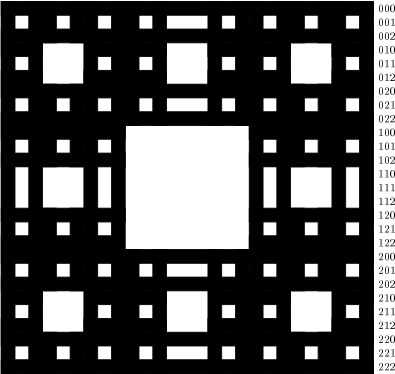
\includegraphics{images/menger-schema05.png}
\end{center}
\item [\textbullet] \textbf{Dernière étape:} On s'intéresse alors aux lignes dont le numéro comporte deux 1 placés aux premières positions. On trace successivement par alternance des rectangles en suivant le schéma $[3\ 3\ 3\ 9\ 3\ 3\ 3]$. On reporte ensuite cette opération sur les colonnes.
\begin{center}
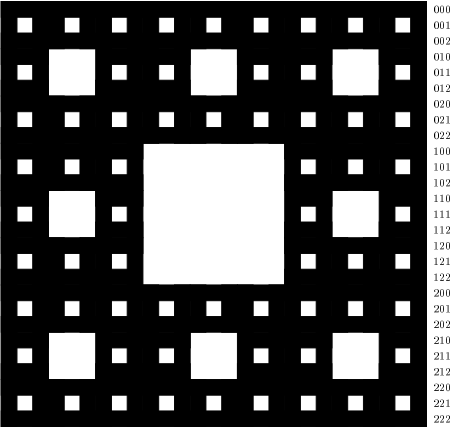
\includegraphics{images/menger-schema06.png}
\end{center}
\end{itemize}
La construction du tapis de Sierpinski d'ordre 3 est alors terminée. Pour créer ce tapis, il a fallu utiliser en tout: $16+16+32+16=80$ polygones.
\subsection{Différents schémas de colonnes possibles}
Pour récapituler la construction précédente, voici les différents types de schémas de colonnes suivant leur numéro de lignes. (Le symbole * désigne le chiffre 0 ou le chiffre 2)
\begin{center}
 \begin{tabular}{|c|c|}
 \hline
Numéro de ligne du type & Schéma à appliquer \\
\hline
*** & 27 \\ 
\hline
1** &  9 9 9 \\
\hline
*1* & 3 3 6 3 6 3 3\\
\hline
11* & 3 3 3 9 3 3 3\\
\hline
\end{tabular}
\end{center}

Sur le même principe, pour créer un tapis d'ordre 4, on utilisera un carré avec $3^4=81$ carreaux. Les numéros de ligne et de colonne possèderont donc 4 chiffres dans leur décomposition en base 3. Pour chaque type de numéro de lignes, voici le schéma à appliquer (le symbole * désigne le chiffre 0 ou le chiffre 2):
\begin{center}
 \begin{tabular}{|c|c|}
 \hline
Numéro de ligne du type & Schéma à appliquer \\
\hline
 **** & 81 \\ 
\hline
1*** &  27 27 27 \\
\hline
*1** & 9 9 18 9 18 9 9 \\
\hline
**1* & 3 3 6 3 6 3 6 3 6 3 6 3 6 3 6 3 6 3 3 \\
\hline
*11* &  3 3 3 9 3 3 6 3 3 9 3 3 6 3 3 9 3 3 3 \\
\hline
1*1* & 3 3 6 3 6 3 3 27 3 3 6 3 6 3 3 \\
\hline
11** & 9 9 9 27 9 9 9 \\
\hline
111*& 3 3 3 9 3 3 3 27 3 3 3 9 3 3 3 \\
\hline
\end{tabular}\\
496 polygônes sont alors nécessaires pour tracer un tapis de Sierpinski d'ordre 4.\\
\end{center}
Enfin, voici les chémas de constructions de colonnes pour les solides d'ordre 2:
\begin{center}
  \begin{tabular}{|c|c|}
 \hline
Numéro de ligne du type & Schéma à appliquer \\
\hline
** &  9 \\
\hline
1* & 3 3 3 \\ 
\hline
\end{tabular}
\end{center}
\subsection{Le programme}
\begin{verbatim}
 #trace un tapis de Sierpinski d'ordre :p et de taille :size
pour carpet :size :p
donne "unit :size/(puissance 3 :p)
si :p=0 [ rec :size :size stop]
si :p=1 [repete 4 [rec :size :unit av :size td 90 ] stop]
repetepour (liste "x 1 puissance 3 :p) [
  soit "cantorx cantor :x :p []
# On ne trace pas les éléments ayant un 1 en derniere position
si  non (1=dernier :cantorx)  [
  soit "nom evalue saufdernier :cantorx "
  drawColumn :x rprop "map :nom
  ]
]  
fin

# Retourne la décomposition en base 3 du nombre x
# p indice de profondeur 3^p
# :list liste vide au démarrage

pour cantor :x :p :list
si :p=0 [retourne :list] 
soit "a puissance 3 :p-1
si :x<= :a [
  retourne cantor  :x :p-1  phrase :list 0] 
  [ si :x<=2*:a [retourne cantor  :x-:a :p-1  phrase :list 1] 
  retourne cantor :x-2*:a :p-1 phrase :list 0]
fin

# Trace la colonne numéro x en respectant le schéma de construction défini dans la liste
pour drawcolumn :x :list
  lc  td 90 av (:x-1)*:unit tg 90  bc des :list
  lc tg 90 av (:x-1)*:unit td 90 av :x*:unit td 90 bc des :list
lc tg 90 re :x*:unit bc
fin

# Trace un rectangle de dimensions données
# Le polygone est enregistrées par le viewer3d
pour rec :lo :la
donne "compteur :compteur+1
polydef
repete 2 [av :lo td 90 av :la td 90]
polyfin
fin

# Initialise les différentes colonnes possibles pour les tapis d'ordre 1 à 4
pour initmap
dprop "map 111 [3 3 3 9 3 3 3 27 3 3 3 9 3 3 3]
dprop "map 110 [9 9 9 27 9 9 9]
dprop "map 101 [3 3 6 3 6 3 3 27 3 3 6 3 6 3 3]
dprop "map 011 [3 3 3 9 3 3 6 3 3 9 3 3 6 3 3 9 3 3 3]
dprop "map 000 [81]
dprop "map 100 [27 27 27]
dprop "map 010 [9 9 18 9 18 9 9]
dprop "map 001 [3 3 6 3 6 3 6 3 6 3 6 3 6 3 6 3 6 3 3]
dprop "map 01 [3 3 6 3 6 3 3]
dprop "map 00 [27]
dprop "map 10 [9 9 9]
dprop "map 11 [3 3 3 9 3 3 3]
dprop "map 1 [3 3 3]
dprop "map 0 [9]
fin

# Si la decomposition est [1 0 1] --> retourne 101
pour evalue :list :mot
  si vide? :list [retourne :mot]
  [
  soit "mot mot :mot premier :list
  retourne evalue saufpremier :list :mot  
]
fin
# Trace les blocs de rectangles de chaque colonne par alternance
pour des :list
soit "somme 0
repetepour (liste "i 1 compte :list) [
   soit "element item :i :list
    soit "somme :element+:somme 
  si pair? :i [lc av :element*:unit bc ] [rec :element*:unit :unit av :element*:unit]  
]
lc re  :somme * :unit bc
fin

# Teste si un nombre est pair
pour pair? :i
retourne 0=reste :i 2
fin

pour tapis :p
ve perspective ct initMap
donne "compteur 0
carpet 810 :p
tape "Nombre\ de\ polygones:\  ec :compteur 
vue3d
fin
\end{verbatim}
\texttt{tapis 3} dessine un tapis de Sierpinski d'ordre 3 de côté 810. Voilà, nous sommes prêts à passer à l'éponge de Menger!

\subsection{L'éponge de Menger d'ordre 4}
L'éponge de Menger possède de multiples propriétés de symétrie. Pour la générer nous allons tracer les différentes sections suivant le plan $(xOy)$ puis reporter ces figures suivant $(yOz)$ et $(xOz)$. Pour bien expliquer ce qui se passe, restons sur l'exemple de l'éponge d'ordre 3:\\
Lorsque l'on coupe l'éponge par un plan vertical, on peut obtenir quatre motifs différents:\\
\vspace*{0.6cm}
 \begin{center}
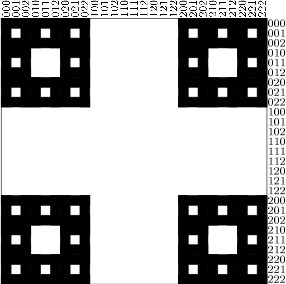
\includegraphics{images/menger-schema07.png}\\ \vspace{0.5cm}
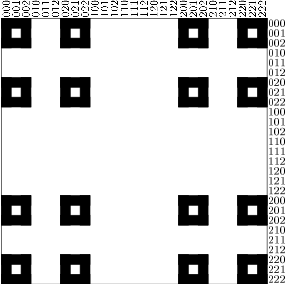
\includegraphics{images/menger-schema08.png}\\ \vspace{0.5cm}
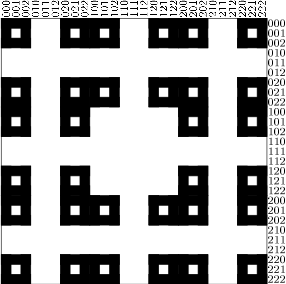
\includegraphics{images/menger-schema09.png}\\ \vspace{0.5cm}
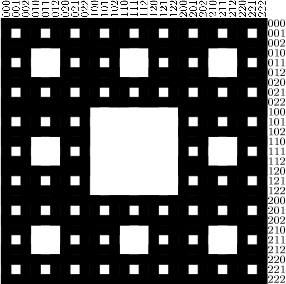
\includegraphics{images/menger-schema10.png}\\ 
\end{center}
Pour tracer une éponge d'ordre 3, nous allons parcourir les nombres de 1 à 27, c'est à dire de 001 à 222 en base 3. Pour chaque numéro, on appliquera la section adéquate que l'on reportera suivant les 3 directions $(Ox)$, $(Oy)$ et $(Oz)$.
\subsubsection{Le code}
\noindent Le programme suivant permet de tracer les solides de Menger d'ordre 0,1,2,3,4. Le nombre de procédures est important donc j'apporterai quelques éclaircissements ensuite.
\begin{verbatim}
#trace un tapis de Sierpinski d'ordre :p et de taille :size
pour carpet :size :p
donne "unit :size/(puissance 3 :p)
si :p=0 [ rec :size :size stop]
si :p=1 [repete 4 [rec :size :unit av :size td 90 ] stop]
repetepour (liste "x 1 puissance 3 :p) [
  soit "cantorx cantor :x :p []
# On ne trace pas les éléments ayant un 1 en derniere position
si  non (1=dernier :cantorx)  [
  soit "nom evalue saufdernier :cantorx "
  drawColumn :x rprop "map :nom
  ]
]  
fin

# Retourne la décomposition en base 3 du nombre x
# p indice de profondeur 3^p
# :list liste vide au démarrage

pour cantor :x :p :list
si :p=0 [retourne :list] 
soit "a puissance 3 :p-1
si :x<= :a [
  retourne cantor  :x :p-1  phrase :list 0] 
  [ si :x<=2*:a [retourne cantor  :x-:a :p-1  phrase :list 1] 
  retourne cantor :x-2*:a :p-1 phrase :list 2]
fin

# Trace la colonne number x en respectant le schéma de construction défini dans la liste
pour drawcolumn :x :list
  lc  td 90 av (:x-1)*:unit tg 90  bc des :list
  lc tg 90 av (:x-1)*:unit td 90 av :x*:unit td 90 bc des :list
lc tg 90 re :x*:unit bc
fin

# Trace un rectangle de dimensions données
# Le polygone est enregistrées par le viewer3d
pour rec :lo :la
donne "compteur :compteur+1
polydef
repete 2 [av :lo td 90 av :la td 90]
polyfin
fin

# Initialise les différentes colonnes possibles pour les tapis d'ordre 1 à 4
pour initmap
dprop "map 111 [3 3 3 9 3 3 3 27 3 3 3 9 3 3 3]
dprop "map 110 [9 9 9 27 9 9 9]
dprop "map 101 [3 3 6 3 6 3 3 27 3 3 6 3 6 3 3]
dprop "map 011 [3 3 3 9 3 3 6 3 3 9 3 3 6 3 3 9 3 3 3]
dprop "map 000 [81]
dprop "map 100 [27 27 27]
dprop "map 010 [9 9 18 9 18 9 9]
dprop "map 001 [3 3 6 3 6 3 6 3 6 3 6 3 6 3 6 3 6 3 3]
dprop "map 01 [3 3 6 3 6 3 3]
dprop "map 00 [27]
dprop "map 10 [9 9 9]
dprop "map 11 [3 3 3 9 3 3 3]
dprop "map 1 [3 3 3]
dprop "map 0 [9]
fin

# Si la decomposition est [1 0 1] --> retourne 101
# Si la decomposition est [1 0 2] --> retourne 100
#  Les éléments de la liste sont concaténés en un mot. 
# De plus, es 2 sont remplacés par des zéros
pour evalue :list :mot
  si vide? :list [retourne :mot]
  [
  soit "first premier :list
  si :first=2 [soit "first 0] 
 soit "mot mot :mot :first
  retourne evalue saufpremier :list :mot  
]
fin
# Trace les blocs de rectangles de chaque colonne par alternance
pour des :list
soit "somme 0
repetepour (liste "i 1 compte :list) [
   soit "element item :i :list
    soit "somme :element+:somme 
  si pair? :i [lc av :element*:unit bc ] [rec :element*:unit :unit av :element*:unit]  
]
lc re  :somme * :unit bc
fin

# Teste si un nombre est pair
pour pair? :i
retourne 0=reste :i 2
fin

pour tapis :p
ve perspective ct initMap
donne "compteur 0
carpet 810 :p
tape "Nombre\ de\ polygones:\  ec :compteur 
vue3d
fin

# Supprime le dernier 1 dans la liste :list
pour deletelastone :list
repetepour (liste "i compte :list 1 moins 1) [
  soit "element item :i :list 
  si :element=1 [soit "list remplace :list :i 0 stop] [si :element=2 [stop]]
]
retourne :list
fin

# Eponge de Menger de taille donnée et de profondeur :p

pour menger :size :p
donne "unite :size/(puissance 3 :p)
repetepour (liste "z 1 puissance 3 :p) [
  soit "cantorz cantor :z :p []
  soit "last dernier :cantorz
  soit "cantorz saufdernier :cantorz
  si :last=0 [soit "order evalue deleteLastOne :cantorz "]  [soit "order evalue :cantorz "]
  soit "order mot "coupe :order
  draw3carpet :size :order :z
  lc cabre 90 av :unit pique 90 bc 
]
draw3carpet :size :order (puissance 3 :p)+1
fin

# Trace les tapis de Sierpinski d'ordre :p
# suivant chaque axe (Ox), (Oy) et (Oz)
# à l'altitude :z
pour draw3carpet :size :order :z
lc origine  
cabre 90 av (:z-1)*:unite pique 90 bc
fcc bleu exec :order :size
lc origine  
rg 90 av (:z-1)*:unite pique 90  bc
fcc jaune exec :order :size
lc origine  
cabre 90 av :size td 90 av (:z-1)*:unite pique 90 bc
fcc magenta exec :order :size 
fin


# Procédure principale
# Trace une eponge de Menger de profondeur p
pour eponge :p
ve perspective ct
soit "temps temps
initMap
donne "compteur 0
si :p=0 [cube 405] [menger 405 :p]
# Affiche le temps mis et le nombre de polygone nécessaire à la construction
tape "Nombre\ de\ polygones:\  ec :compteur 
tape "Temps\ mis:\  ec temps -:temps 
vue3d
fin

# Section pour le Menger d'ordre 2
pour coupe1 :size
repete 4 [carpet :size/3 1 lc av :size td 90 bc]
fin

pour coupe0 :size
carpet :size 2
fin

# Section pour le Menger d'ordre 3

pour coupe10 :size
repete 4 [carpet :size/3 2 lc av :size td 90 bc]
fin

pour coupe01 :size
repete 4 [repete 2 [coupe1 :size/3 lc av :size/3 bc] av :size/3 td 90]
fin

pour coupe11 :size
repete 4 [coupe1 :size/3 lc av :size td 90 bc]
fin


pour coupe00 :size
carpet :size 3
fin

# Section pour le Menger d'ordre 4
pour coupe000 :size
carpet :size 4
fin

pour coupe100 :size
repete 4 [carpet :size/3 3 lc av :size td 90 bc]
fin

pour coupe010 :size
repete 4 [repete 2 [coupe10 :size/3 lc av :size/3 bc] av :size/3 td 90]
fin

pour coupe001 :size
repete 4 [repete 2 [coupe01 :size/3 lc av :size/3 bc] av :size/3 td 90]
fin

pour coupe110 :size
repete 4 [coupe10 :size/3 lc av :size bc td 90 ]
fin

pour coupe111 :size
repete 4 [coupe11 :size/3 lc av :size td 90 bc]
fin

pour coupe101 :size
repete 4 [coupe01 :size/3 lc av :size td 90 bc]
fin

pour coupe011 :size
repete 4 [repete 2 [coupe11 :size/3 lc av :size/3 bc] av :size/3 td 90]
fin

pour coupe :size
carpet :size 1
fin

pour cube :size
repete 2 [
fcc bleu rec :size :size lc av :size pique 90 bc 
fcc jaune rec :size :size lc av :size pique 90  bc
]
fcc magenta
lc rg 90 tg 90 av :size td 90 bc rec :size :size
lc td 90 av :size tg 90 rd 90 td 90 av :size tg 90 rd 90 bc rec :size  :size
rg 90 tg 90 av :size td 90
fin

pour cubes
ve perspective ct
soit "temps temps
initMap
donne "compteur 0
repete 4 [si compteur=1 [cube 405] [menger 405 compteur-1] lc av 1000 td 90 bc ]
# Affiche le temps mis et le nombre de polygone nécessaire à la construction
tape "Nombre\ de\ polygones:\  ec :compteur 
tape "Temps\ mis:\  ec temps -:temps 
vue3d
fin
\end{verbatim}
Ensuite, on règle la mémoire allouée à \xlogo\ à 640 Mo: \texttt{eponge 4}
\begin{center}
 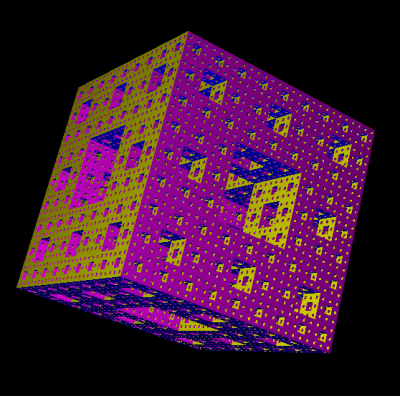
\includegraphics{images/menger-menger4.png}
\end{center}